% So we make this "beamer" rather than document!

\documentclass[11pt]{beamer}
% For handout add ,handout after 11pt
% Kill page numbers with [numbering=none] in next line:
\usetheme[sectionpage=none,numbering=none]{metropolis}           % Use metropolis theme
	% To do printouts, add ", handout"  after aspectratio.
\usepackage{makecell}
\usepackage{booktabs}
\usepackage{graphicx}
\usepackage{color}
%\usepackage[utf-8]{inputenc}
\usepackage{bbm}
  \usepackage{bm}
\newcommand{\notimplies}{%
  \mathrel{{\ooalign{\hidewidth$\not\phantom{=}$\hidewidth\cr$\implies$}}}}
\definecolor{violet}{RGB}{223,115,255}
\usepackage{transparent}
\definecolor{cyan2}{RGB}{0,255,255}
\makeatletter
\newcommand\primitiveinput[1]
{\@@input #1 }
\makeatother
\usepackage{tabu}
\usepackage{dcolumn}
\definecolor{Gray}{gray}{0.85}

\usepackage{xcolor,colortbl}


\title{Practical Data Science: \\ Wrangling Data and Answering Questions}
\author{\small Nick Eubank}
\date{\vspace*{.3in} \date}


% This is the beginning of a real document!
\begin{document}


\begin{frame}
\maketitle
\end{frame}


\begin{frame}[c]{What is Data Science?}
\begin{enumerate}
	\pause \item What (\alert{in theory}) do we think Data Science should be?
	\pause \item What (\alert{empirically}) is Data Science?
\end{enumerate}
\end{frame}


\begin{frame}[c]{What (in theory) should Data Science be?}

\pause Discipline of learning how best to \alert{answer questions} using \alert{quantitative data.}

\pause
\begin{itemize}
	\item Question-first approach \\
	\pause The tool you use should be dictated by the answer you seek to answer
\end{itemize}

\end{frame}

\begin{frame}[c]{What (empirically) is Data Science?}

\end{frame}

\begin{frame}[c]{Where are we today?}

Over the past several decades:
\begin{enumerate}
	\item Availability of data $\uparrow$
	\item Computational power $\uparrow$
\end{enumerate}
\pause
$\Rightarrow$ Huge proliferation and increase in sophistication of computational methods
\end{frame}


\begin{frame}[c]{Where are we today?}

\begin{itemize}
	\item Academic research is organized into silos:
	\pause
	\begin{itemize}
		\item Computer Science
		\item Statistics
		\item Economics
		\item Political science
		\item Engineering
	\end{itemize}
\end{itemize}
$\Rightarrow$ Development of new tools occurred \emph{within} each silo.
\end{frame}


\begin{frame}[c]{Where are we today?}
Problems:
\begin{itemize}
	\pause \item Very little cross-pollination across silos, lots of duplication of development.
	\pause \item Each silo has focused on the aspects most relevant to their applications. e.g.:
	\begin{itemize}
		\pause \item CS likes to classify things and make predictions, don't care how model works
		\item Social scientists like to make causal statements, don't care about predictive power
	\end{itemize}
	\pause \item Every silo has its own vocabulary, \emph{even when talking about the same thing}.
\end{itemize}
\end{frame}

\begin{frame}[c]{}
\pause 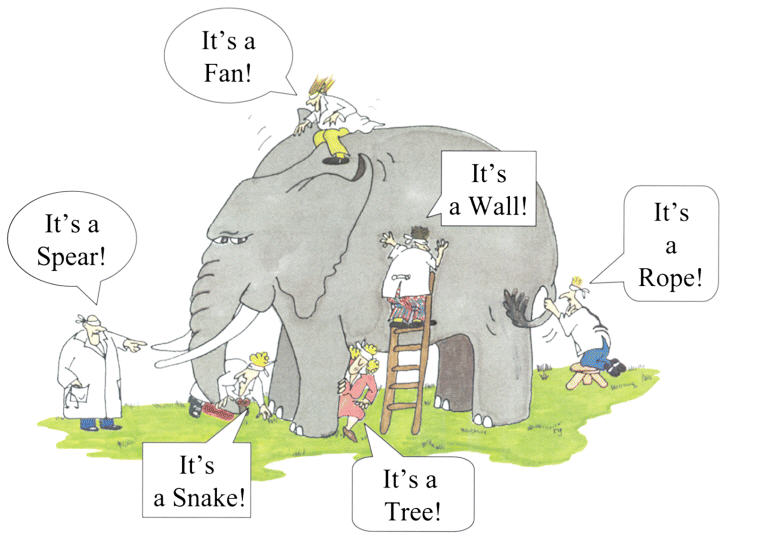
\includegraphics[width=\textwidth]{blindmenelephant.jpg}
\pause $\Rightarrow$ This is where we are \emph{now.}
\end{frame}

\begin{frame}[c]{What is (empirically) Data Science?}
\pause An effort to unify the development of quantitative methods \\
\pause $\rightarrow$ Recognize the elephant
\end{frame}

\begin{frame}[c]{Why does this matter to you?}
\begin{itemize}
	\item Most current researchers learned their skills in a silos. \\
	\pause In many ways, \alert{\emph{you} will have better perspective than your professors.}
	\item Important not just technically, but also when it comes to advice.
	\begin{itemize}
		\pause \item Recognize that your professors' conception of ``data science'' \alert{may not match yours}.
		\pause \item Also just good life advice: scientists are \alert{very unscientific} when it comes to career advice!
	\end{itemize}
\end{itemize}
\end{frame}

\begin{frame}[c]{Areas of Data Science}
	\begin{columns}
	\begin{column}{0.45\textwidth}
		\uncover<1->{\textbf{Software Engineering DS}}
		\begin{itemize}
			\item \uncover<2->{Recommendation engines}
			\item \uncover<2->{Financial trading algorithms}
			\item \uncover<2->{Self-driving cars}
		\end{itemize}
	\end{column}
	\begin{column}{0.5\textwidth}  %%<--- here
		\uncover<1->{\textbf{Data Analysis DS}}
		\begin{itemize}
			\item \uncover<3->{Impact of policy change}
			\item \uncover<3->{Effectiveness of health interventions}
			\item \uncover<3->{Plan political campaigns}
		\end{itemize}
	\end{column}
	\end{columns}
	\vspace*{1cm}
\uncover<4->{Nearly all data scientists will use some of both sets of skills.}\\
\uncover<5->{In this class, we will be focused on the \alert{Data Analysis} flavor of Data Science.}
\end{frame}


\begin{frame}[c]{This Class}
\begin{itemize}
	\item Flipped Classroom
\end{itemize}
\end{frame}

\begin{frame}[c]{About Me}
	I am a social scientist \\
	\vspace{0.5cm}
	\begin{itemize}
		\pause \item PhD in Political Economy
		\pause \item Master in Economics
		\pause \item BA in Economics and Political Science
	\end{itemize}
\end{frame}

\begin{frame}[c]{My Research}
	\begin{itemize}
		\pause \item Looking for evidence of polling place manipulation in North Carolina
		\pause \item Developing methods of measuring Gerrymandering in the US.
		\pause \item Testing theories about how social networks shape political behavior using cell-phone meta-data to map social networks of entire countries (Zambia and Venezuela).
		\pause \item Studying whether political elites in the US South turned to using incarceration to prevent black voters from exercising political influence after the Voting Rights Act removed their ability to use Jim Crow restrictions.
	\end{itemize}
\end{frame}

\begin{frame}[c]{What that means for you}
\pause I've worked with \emph{a lot} of messy data in many contexts. \\
\pause I have unusually broad exposure to data science:
\begin{itemize}
	\pause \item Within academic circles, I've worked with economists, statisticians, computer scientists, and political scientists.
	\pause \item I've done \alert{policy consulting} (World Bank, Center for Global Development), \alert{public outreach} (Op-Ed in \emph{The Guardian}), and \alert{legal consulting} (various voting rights cases).
\end{itemize}
\pause \emph{If} this sounds like your ``flavor'' of data science, I'm happy to talk about career options in this domain.
\end{frame}



\end{document}
